\documentclass[Interploate_hadwritten_Digits.tex]{subfiles}

\begin{document}
	\subsection{Aufbereitung der Daten}
	Als Datensatz wurde der MNIST Datensatz von der offiziellen Webseite\footnote{ http://yann.lecun.com/exdb/mnist/} von Yann LeCun verwendet. Dieser Umfasst ein Trainingsset von \numprint{60000} und ein Testset von \numprint{10000} gelabelten Datensätzen in jeweils zwei verschiedenen Dateien, eine für die Bilder und eine für die Labels. Von der Bilder-Datei werden die jeweils 28x28 Bytes eingelesen und in einen 784-dimensionalen Vektor eingelesen. Dabei werden die Werte auf Float-Werte zwischen Null und Eins verwandelt. Die Label-Datei wird Byteweise eingelesen und in eine One-Hot Vektor der Länge zehn verwandelt, bei welchem der Index der Eins dem Wert des Labels entspricht. 
	
	\subsection{Das Modell erstellen und trainieren}
	Das Neuronale Netz wurde mit Tensorflow\footnote{https://www.tensorflow.org} modelliert und trainiert. Das verwendete Modell ist ein Feed Forward Neuronal Network mit Weights und Biases für jede Schicht. Um den Output des Netzes zu berechnen, muss $ \vec{x_{n}} $ berechnet werden, wobei $ x_{0} $ dem Bildvektor entspricht und die restlichen Werte gemäss Gleichung \ref{eq:layer_calculation} berechnet werden. $ n $ entspricht dabei der Anzahl Schichten im Neuronalen Netz.
	\begin{equation}
	\vec{x_{i}} = a(\vec{x_{i-1}} \times w_{i-1} + b_{i-1})
	\label{eq:layer_calculation}
	\end{equation}
	
	Als Aktivierungsfunktion $ a(x) $ wird die Logistische Sigmoidfunktion (siehe Gleichung \ref{eq:sigmoid}) verwendet, welche auf alle Elemente im Vektor angewendet wird. 
	\begin{equation}
	f(x)=\frac{1}{1+e^{-x}}
	\label{eq:sigmoid}
	\end{equation}
	Sie hat die Aufgabe zu verhindern, dass Zahlen durch die Multiplikationen zu gross oder zu klein werden. Dies erreicht die Funktion in dem sie den Definitionsbereich $ [-\infty, \infty] $ auf den Wertebereich $ [0, 1] $ einschränkt. Dieses Verhalten ist in der Abbildung \ref{fig:sigmoid_plot} visualisiert.
	\begin{Figure}
		\centering
		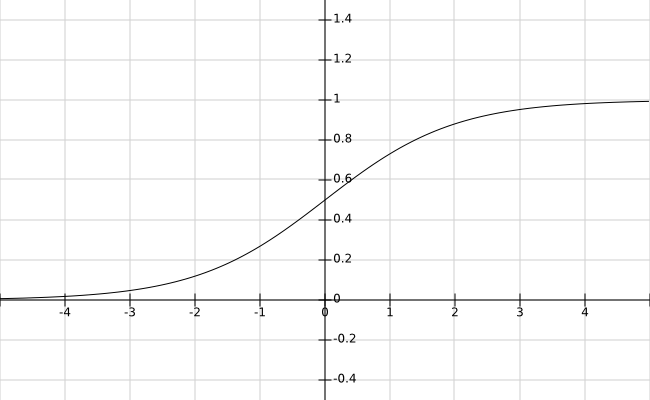
\includegraphics[width=\linewidth]{img/sigmoid_plot.png}
		\captionof{figure}{Verhalten der Sigmoid Funktion}
		\label{fig:sigmoid_plot}
	\end{Figure}

	Der Fehler des Netzwerks wird durch die Kreuzentropie (Gleichung \ref{eq:cross_entropy}) zwischen dem normalisierten Output-Vektors $ \vec{x} $ des Neuronalen Netzes und dem Label-Vektor $ \vec{y} $ berechnet.
	\begin{equation}
	H(\vec{x}, \vec{y}) = -\sum_{n}^{k}x_{k}log(y_{i})
	\label{eq:cross_entropy}
	\end{equation}
	Dabei wird der Output-Vektor des Netzes wird mithilfe der Softmax-Funktion (Gleichung \ref{eq:softmax}) normalisiert. Dadurch liegen alle Werte des Vektors im Bereich $ [0, 1] $ und die Länge des Vektors wird eins. Dieser Vektor kann als diskrete Wahrscheinlichkeitsverteilung für das Erkennen der Ziffer im Input-Vektor betrachtet werden.
	\begin{equation}
	\sigma(v)_{i} = \frac{e^{v_{i}}}{\sum_{n}^{k=1}e^{v_{k}}}
	\label{eq:softmax}
	\end{equation}
	
	Für die Korrektur des Fehlers im Neuronalen Netz wird ein Gradientenverfahren eingesetzt um den über die Kreuzentropie berechneten Fehler zu minimieren. In diesem Verfahren wird die Ableitung des Modelles bestimmt und jeder Parameter, in diesem Fall die Weight- und Bias-Matrizen, um einen bestimmten Betrag in die Richtung des steilsten Abfalls korrigiert. Der Korrekturbetrag ergibt sich aus der Steigung am Punkt der Ableitung und dem Hyperparameter der Learning Rate.
	\begin{equation}
	b = a - \gamma \Delta f(a)
	\label{eq:gradient_decent}
	\end{equation}
	Das grundlegende Konzept des Gradientenverfahren kann der Gleichung \ref{eq:gradient_decent} entnommen werden. Der neue Wert $ b $ ergibt sich aus dem Lerning Rate $ \gamma $ multipliziert mit der Richtung des steilsten Abfalls $ \Delta f(a) $ subtrahiert vom ursprünglichen Wert $ a $.
	
	\subsection{Rückrechnung im Neuronalen Netz}
	Um die Funktion des Neuronalen Netzes zu invertieren wurde in einem ersten Schritt eine komprimierte Version dieses Netzes erstellt. Diese Komprimierung bestand darin, wie in Gleichung \ref{eq:homogenize_layer} beschrieben die Weight- und Bias-Matrizen in den homogenen Raum zu transformieren und so die Addition des Bias-Vektors und die Multiplikation der Weight-Matrix in eine Matrix pro Layer zusammenzunehmen.
	\begin{equation}
		M_{i} =
		\begin{bmatrix}
		I & \vec{b_{i}} \\ 
		\vec{0}^{T} & 1
		\end{bmatrix}
		\times
		\begin{bmatrix}
		w_{i} & \vec{0} \\ 
		\vec{0}^{T} & 1 
		\end{bmatrix}
		\label{eq:homogenize_layer}
	\end{equation}
	
	Als nächster Schritt wurde versucht, die Matrizen aller Layers in eine zusammenzuführen, welche mit dem Inputvektor multipliziert werden kann und so die Schritte im Neuronalen Netz auf eine Matrixmultiplikation reduziet. Dies wurde gemäss der Gleichung \ref{eq:network_compression} gemacht. Dabei wurde angenommen, dass die Aktivierungsfunktion auf das Produkt der Matrixmultiplikation angewendet werden könnte, da deren Funktion das Einschränken des Wertebereichs ist. Diese Annahme erwies sich jedoch als falsch (mehr dazu in Kapitel \ref{sec:results_compression}).
	\begin{equation}
		N_{0} = M_{0},
		N_{i} = a(M_{i} \times N_{i - 1})
		\label{eq:network_compression}
	\end{equation}
	
	Da diese Komprimierung scheiterte, wurde nur die Komprimierung der einzelnen Layers beibehalten. Um das Netz zu invertieren wurde das Pseudoinverse aller Layer-Matrizen $ M_{i} $ berechnet. Da nicht alle Matrizen mit beliebigen Dimensionen besitzen, wird dieses Pseudoinverse lediglich approximiert. Gemäss der Dokumentation der verwendeten Library\footnote{ https://docs.scipy.org/doc/numpy-1.15.1/reference/generated/numpy.linalg.pinv.html} wird dies über die KQ-Methode erreicht. Das Inverse des Neuronalen Netzes ist so durch die Gleichung \ref{eq:feed_backwards} gegeben.
	\begin{equation}
		\vec{x_{i}} = a(M_{n-i}^{+} \times \vec{x_{i-1}})^{-1}
		\label{eq:feed_backwards}
	\end{equation}
	Dabei ist $ a(x)^{-1} $ das inverse der Aktiverungsfunktion und definiert durch die Gleichung \ref{eq:sigmoid_inverse}.
	\begin{equation}
		a(x)^{-1} = log_{e}(\frac{1}{x - 1})
		\label{eq:sigmoid_inverse}
	\end{equation}
	
	Da das Pseudoinverse nicht garantiert ein echtes Invers ist, könnte die einen Einfluss auf die Resultate haben. Aus diesem Grund wurde ein weiteres Neuronales Netz trainiert, welches dasselbe Modell verwendet, jedoch die Dimensionen nicht verändert. So konnte sichergestellt werden, dass alle Matrizen $ M_{i} $ im komprimierten Netz quadratisch sind und es so auch ein echtes Invers gibt.
	
	\subsection{Approximation von Input Bildern}
	Bei der Evaluation der Funktionalität des invertieren Neuronalen Netzes konnte eine mögliche Fehlerquelle für verfälschte Resultate ausfindig gemacht werden: Die in der Regel insignifikante Inpräzision von Gleitkommazahlen in Computern wurde durch das Inverse der Sigmoidfunktion verstärkt und in einen signifikanten Bereich gebracht. Um diese Fehlerquelle zu umgehen wurde ein weiteres Neuronales Netz trainiert. Dieses Neuronale Netz verwendet das gleiche Modell wie das Netz, welches zur Erkennung handgeschriebener Ziffern trainiert wurde, mit dem Unterscheid dass die Weigth- und Bias-Matrizen als Konstanten definiert wurden. Als variabler Teil für die Optimierung wurde eine zufällig initialisierte Matrix definiert, welche im alten Model für das Inputbild stand. In diesem Modell sucht das Gradientenverfahren ein Inputbild, welches möglichst nahe am Bild ist, welches den gesuchten Vektor im Zielraum entspricht.
	
\end{document}